\section{Abstract}

This report investigates the feasibility of stock price prediction using news article sentiment. Presented is an overview of the issue, a comparison oif various textual sources, a literature review of the subject, and the detailing of development of a machine learning model to predict stock price movements, integrating sentiments and features extracted from smallcaps articles. This report presents a pipeline that collects news articles using web scraping techniques and processes them through NLP systems to extract meaningful insights. All code and reporting files are available on \href{https://github.com/H-unter/MA3831-Assignment-2-3}{GitHub}. 

\section{Introduction}

% MUST INCLUDE
% an overview of the issue
% where the issue is present on the web(research literature review)
% how machine learning can be applied to provide a solution

Predicting the movements of the stock market is a long standing challenge. Its erratic and volatile nature leads many to believe that predicting it is a fools game, with even experts in the field unable to consistently outperform the market \cite{efh_article,swedroe_spiva,gunnars2024beatmarket}. 

Many efforts have been made to predict stock price movements, with a variety of methods employed, with machine learning being particularly popular in recent years \cite{al_literature_review}. A literature review conducted by \cite{al_literature_review} analysed 81 papers  from January 2015 to June 2020. This literature review found that support vector machines (SVM) were the most popular method of stock price prediction, with 26.13\% of the analysed papers using them, followed by random forest (RF) (15.32\%), and long short term memory (LSTM) (13.51\%) (\cref{fig:pie_chart_model}). 


The Efficient Market Hypothesis (EMH) claims that asset prices quickly reflect all available information \cite{efh_article}; it is also believed herd behavior and emotions can drive price swings beyond fundamentals \cite{greyling_sentiment}. It therefore follows that incorerating information and sentiment from sources across the internet may improve the performance of stock price prediction models to addess this age old problem. Online financial discourse is heavily concentrated across a few key domains, including social platforms (e.g., Reddit's r/WallStreetBets), news aggregators (e.g., Yahoo Finance), and article-based financial outlets (e.g., Bloomberg), and market announcements \cite{asx_market_announcements}. These domains offer continuous textual data that offer differing levels of up to date information and consumer sentiment. \Cref{fig:pie_chart_data_source} shows that a vast majority of the studies analysed in the literature review by \cite{al_literature_review} used only techincal indicators, and not taking advantage of news data - showing a potential opportunity to explore this field \note{unsure about this sentence}

\begin{figure}[htbp]
    \centering
    \begin{minipage}{0.45\textwidth}
        \centering
        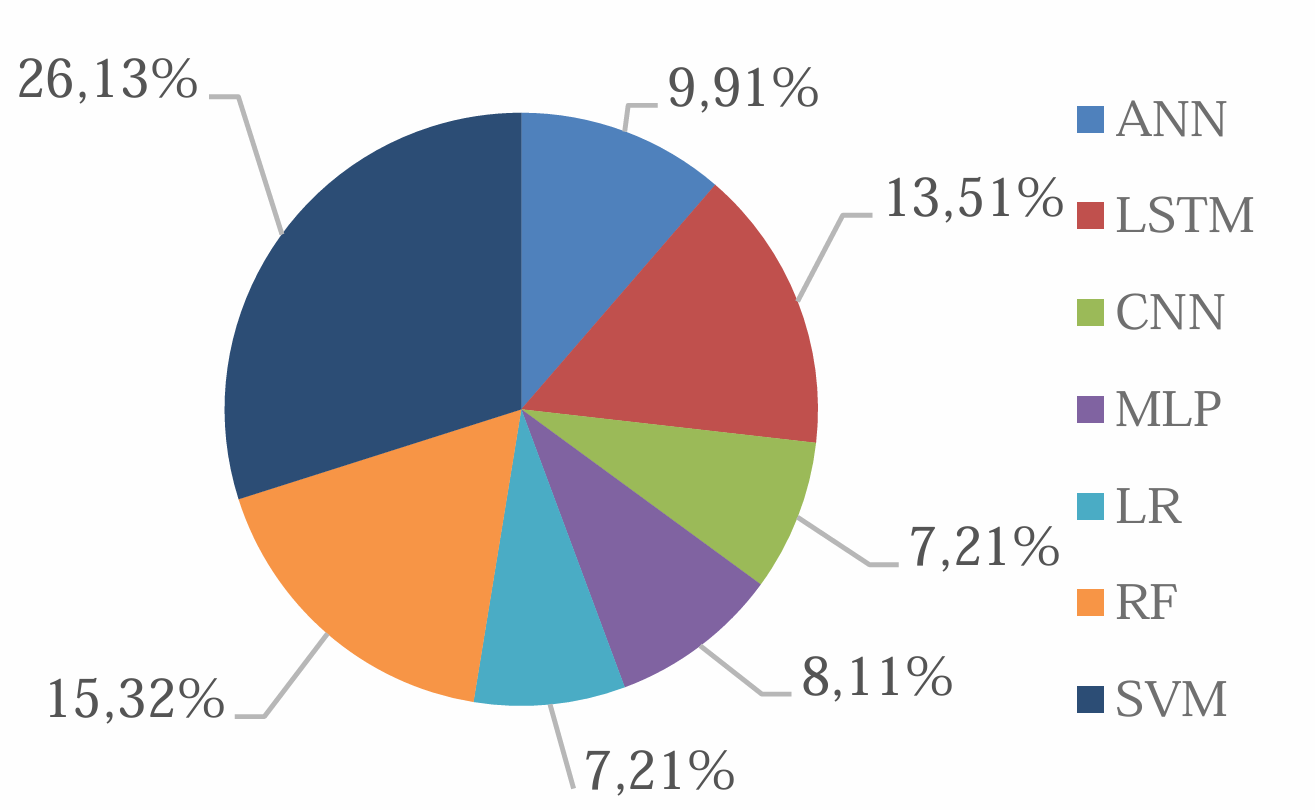
\includegraphics[width=\linewidth]{figures/literature_review_model_proportions.png}
        \caption{Proportion of Each Stock Price Prediction method \cite{al_literature_review}}
        \label{fig:pie_chart_model}
    \end{minipage}\hfill
    \begin{minipage}{0.45\textwidth}
        \centering
        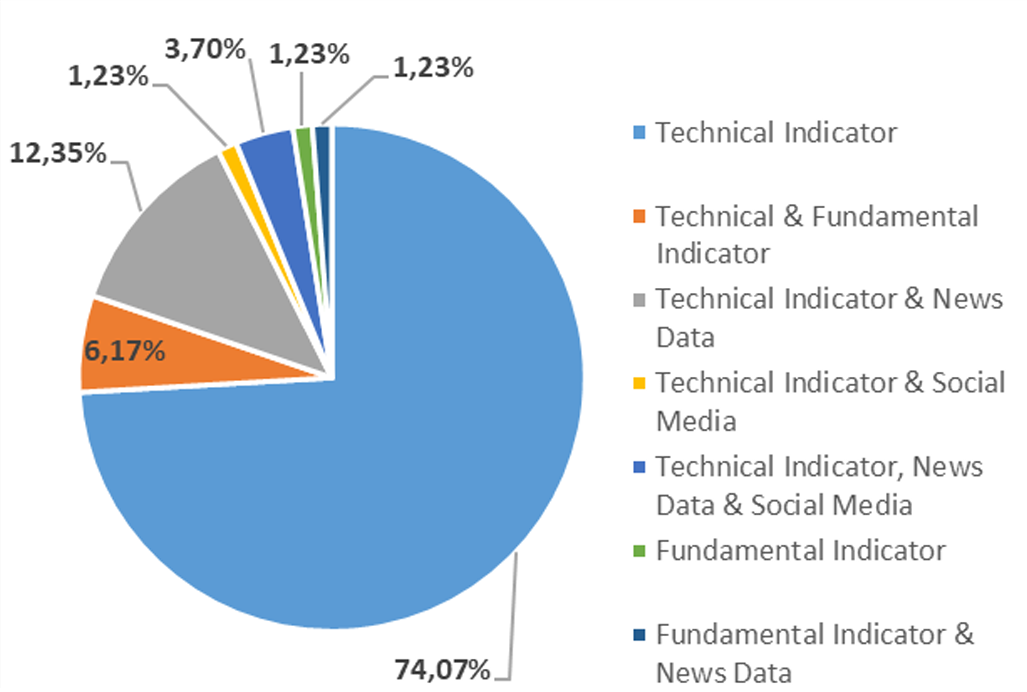
\includegraphics[width=\linewidth]{figures/literature_review_data_source_propotion.png}
        \caption{Proportion of Each of the Studies' Data Source \cite{al_literature_review}}
        \label{fig:pie_chart_data_source}
    \end{minipage}
\end{figure}


% maybe put a table of literature review here




